\documentclass[12pt,a4paper]{article}
\usepackage[a4paper,margin=1.0in]{geometry}
\usepackage{amsmath}
\usepackage{graphicx}
\usepackage{lineno}
%\newcounter{subfigure}
%\usepackage{epstopdf}
\usepackage{color}
\usepackage[normalem]{ulem}
\usepackage[hyphens]{url}
\usepackage{hyperref}
\usepackage{breakurl}
\usepackage{array}
\usepackage{setspace}
\usepackage{multirow}
\usepackage{booktabs}



\setcounter{section}{0}
\renewcommand{\thesection}{S\arabic{section}}
\setcounter{figure}{0}
\renewcommand{\thefigure}{S\arabic{figure}}%
\setcounter{table}{0}
\renewcommand{\thetable}{S\arabic{table}}

\newcommand{\cdigri}{{\ensuremath{^{^\circ}}\mathrm{C}}}
\newcommand{\ndigri}{{\ensuremath{^{^\circ}}\mathrm{N}}}
%\newcommand{\sdigri}{{\ensuremath{^{^\circ}}\mathrm{S}}}
\newcommand{\edigri}{{\ensuremath{^{^\circ}}\mathrm{E}}}
\newcommand{\cms}{{\ensuremath{\mathrm{cm}~\mathrm{s}^{-1}}}}
\newcommand{\chla}{chl-{\emph{a}}}

\usepackage[round]{natbib}
\bibliographystyle{plainnat}


\begin{document}
\begin{center}
\textbf{Supplementary material for}

\vspace{5mm}

\textbf{\Large{Intraseasonal to interannual variability of zooplankton biomass and standing stock inferred from ADCP backscatter in the eastern Arabian Sea}}
  
  \vspace{5mm}

  {R.~K.~Sahu$^{1,2}$, D.~Shankar$^{1,2,*}$, P.~Amol$^{1,3}$, S.~G.~Aparna$^{1,2}$,D.~V.~Desai$^{1,2}$}\\
  
  \vspace{5mm}

\textit{$^1$CSIR National Institute of Oceanography, Dona Paula, Goa-403004, India.} \\
    \textit{$^*$Corresponding author (Email: shankar@nio.res.in)} \\
\textit{$^2$Academy of Scientific and Innovative Research (AcSIR), 
	Ghaziabad, 201002, Uttar~Pradesh, India} \\
\textit{$^3$CSIR-NIO, Regional Centre, Vishakhapatnam, 530017, Andhra Pradesh, India}
  \vspace{5mm}

\end{center}
\linenumbers
	The supplementary material begins with a detailed comparison with the biomass climatology from \citet[A22]{aparna2022seasonal}. This is followed by a section on time-series analysis tools like wavelets and filters. Next, a quality control test is carried out for the Kollam backscatter data during 2020, when unusually low biomass was observed. Finally, additional supplementary figures are included.

\section{Comparison with biomass and zooplankton standing stock (ZSS) climatology of A22}
\label{sec:comparison}
This section compares the climatology of both biomass and Zooplankton Standing Stock (ZSS) from our recent data with those presented in A22 across three overlapping locations: Mumbai, Goa, and Kollam. Both datasets show similar variability in biomass, with peaks associated with the seasonal cycle occurring during winter off Mumbai and summer off Kollam (Fig.~\ref{fig:zsschlclimcomp}a1--c1, a2--c2). The ZSS, integrated from 24~m to 104~m, also exhibits a consistent dip after the summer monsoon, with weaker variability off Kollam (Fig.~\ref{fig:zsschlclimcomp}c1, c2). Despite these similarities, a few differences are evident.


Data from recent years indicate relatively weaker biomass compared to A22, a weakening that extends throughout the water column. This results in the 215 mg m$^{-3}$ biomass contour (D215) being shallower at all three locations, most notably off Goa, where D215, previously aligned with the 23$^\circ$C isotherm ($D23$), now lies approximately 20–40 m shallower during January to April. The overall ZSS also drops due to this biomass weakening, and the timing of maximum or minimum ZSS values doesn't always coincide between the two datasets; for example, the ZSS maximum off Mumbai extends from February in A22 to February–March in the recent data. Off Kollam, the updated ZSS remains almost constant around 25 mg m$^{-2}$, except for a minimum from July to August, whereas A22 shows a gradual biomass drop from March until September followed by an increase. This difference is reflected in a lower correlation between A22's ZSS and the current ZSS climatology off Kollam (0.60) compared to Mumbai (0.94) and Goa (0.98).

Finally, in the present study, chlorophyll-a (Chl-a) peaks across all locations in August, with a smaller peak off Mumbai and Goa, and off Kollam, the mismatch between zooplankton and phytoplankton trends remains consistent with A22's findings (Fig.~\ref{fig:zsschlclimcomp}d1, d2). Climatological values of chlorophyll-a and ZSS are summarized in Table~\ref{table:chl_zss_climatology}.

 
	
% \section{Variability and analysis techniques}
% \label{sec:seasonlity_analysis}
% \subsection{Interannual, annual, and intra-annual variability}
% \label{sec:seasonal_cycle}
%
% Table~\ref{table:biomass_40m_mean_std_range} presents the mean biomass, standard deviation at 40~m and 104~m, and the surface-to-deep biomass difference. Biomass time series exhibits variability across timescales ranging from daily to multi-year periods. The most fundamental pattern is diel vertical migration, characterized by elevated biomass at depth during the day and near the surface at night. On longer timescales, interannual variability driven by changes in monsoon-forced upwelling appears in two forms: (1) quasi-periodic fluctuations with periods $>$400 days, particularly ~600--800 days off Mumbai, Goa, and Kollam (Fig.~9); and (2) aperiodic deviations from the climatological seasonal cycle (Fig.~5).
%
% Annual variability (300--400 days) reflects the dominant seasonal cycle (Fig.\ref{fig:intraannual_annual}, left panels), while intra-annual variability (100--250 days, right panels) captures variation between seasons. In the NEAS, both summer and winter monsoons drive \chla\ blooms, but asymmetries in wind forcing lead to a stronger semi-annual signal \citep{jensen1993equatorial, schott20011} (Fig.~\ref{fig:intraannual_annual}, right; Section~3.2). In the same figure, biomass contours often tilt upward, indicating upward phase propagation in annual band. Though less pronounced than in the annual WICC cycle \citep{amol2014observed, chaudhuri2020observed, chaudhuri2021observed}, this tilt may suggest physical-biological coupling. Such coupling results in phase differences between surface and deep biomass time series. In-phase biomass at both depths enhance column-integrated biomass (e.~g., October--November 2019; Fig.\ref{fig:40_104_biomass_zss}), while phase offsets (e.~g., March--May 2019) yield subdued values. These vertical phase lags, whether between depths or moorings, can be further analyzed using wavelet coherence (Section~\ref{sec:wavelet_analysis}). Intraseasonal variability (5--90 days) arises from short-term environmental changes (Fig.~11), with biomass bursts lasting from a few days to several weeks, much like the intraseasonal current \citep{amol2014observed, chaudhuri2020observed} (Section~5).


\section{Time-series analysis methods}
\label{sec:wavelet_lanczos}

This section describes the time-series analysis tools employed in this study to analyze the biomass data. These tools include wavelets \citep{torrence1998practical}, wavelet coherence \citep{maraun2004cross}, and filters \citep{duchon1979lanczos}.
We used the Python package \texttt{pycwt} for wavelet and wavelet coherence analysis, and the Lanczos function from Ferret for filtering. While commonly used in physical oceanography, such methods are less frequently applied in zooplankton studies due to practical limitations in collecting the extensive time series data required. Unlike traditional biomass data, which are obtained from volumetric zooplankton samples collected from the sea, the biomass data discussed here are derived from hourly ADCP backscatter data extending over 4–6 years. This substantial dataset allows us to investigate zooplankton variability across different timescales, specifically within seasonal and intraseasonal bands, through the application of these tools.




\subsection{Wavelet analysis and wavelet coherence}
\label{sec:wavelet_analysis}

Understanding Fourier analysis lays the groundwork for wavelet analysis. Fourier transforms break down a time series into sine and cosine components. This generates a power spectrum that identifies dominant periodicities, such as annual (360 days) and semi-annual (180 days) cycles.  However, because Fourier analysis assumes signals are constant over time, it can hide changes in non-stationary signals (oscillations whose amplitudes aren't steady), potentially misrepresenting their true strength and variabilities.

Wavelet analysis addresses this limitation and helps identify when oscillating signals are strongest within a time series \citep{torrence1998practical}. For instance, while a Fourier analysis might reveal a dominant 30-day period in biomass data (meaning biomass increases for 15 days and then decreases for 15 days), it won't tell us when these 30-day oscillations actually occur.  Wavelets, however, resolve this. For example, as shown in Figure 6a, wavelet analysis reveals that 30-day oscillations in Okha's data are prominent specifically during the summer monsoon, with color intensity indicating signal strength.

For our study, wavelet analysis is especially useful for detecting both continuous signals, like the annual cycle, and intermittent bursts, particularly within the intraseasonal range. Two key elements guide our interpretation:

\begin{itemize}
\item Cone of Influence (CoI): This shaded area highlights regions where edge effects distort the wavelet results. Since our observations are a finite-length signal, wavelets near the beginning or end of the data lack information outside the observation period and cannot adequately resolve the desired frequency or period near the edges. This distortion is more pronounced for lower frequencies (longer periods) and less so for higher frequencies (shorter periods), creating a cone shape on the plot. The results within the shaded regions of CoI should be interpreted with caution.
\item Statistical Significance Contours: These contours help us determine if a strong peak in the wavelet plot represents a true feature of the underlying signal or just a random fluctuation. To assess this, we use a simple red noise (AR(1) or Markov) model as our null hypothesis, which assumes more power at lower frequencies. In our wavelet figures, the black contour specifically marks the 95\% confidence interval.
\end{itemize}

\noindent For example, in Fig.~6b, the annual signal off Mumbai is both significant and well-contained within the CoI (unshaded region). The figure also reveals significant semi-annual and intraseasonal features.


Wavelet coherence builds on this framework by measuring localized correlations between two time series across both time and frequency \citep{maraun2004cross}. Unlike traditional correlation, it captures time-varying relationships by normalizing the cross-wavelet spectrum, yielding coherence values from 0 to 1. While within-band comparisons are to be interpreted with caution, cross-period comparisons may be biased, particularly at higher periods, due to the normalization scheme \citep{maraun2004cross}. Filtering techniques can mitigate this, enabling reliable variability assessments across distinct bands.

\subsection{Filtering method}
\label{sec:filtering_method}


Filtering techniques are used to isolate variability within a specific frequency band by reducing signals outside that range. For example, when the biomass is filtered using a 5--90-day period band-pass filter, we essentially create a new time series that only contains oscillations between 5 and 90 days. This new time series will precisely tell us when the biomass has reached the maximum or minimum with this band.
Frequency band selection can be based on well-established periods in the region, like the annual cycle, or on prominent periods revealed by wavelet analysis. In this study, our specific choice of frequency bands is motivated by prior research on the West India Coastal Current (WICC), which utilized ADCP data—the source of our backscatter data—at these very locations \citep{amol2014observed, chaudhuri2020observed, chaudhuri2021observed}.


We employed the Lanczos filter, a common choice for oceanographic studies \citep{duchon1979lanczos}. This filter is effective because it minimizes spectral leakage from unwanted signals while preserving the target signal. However, a known limitation of the Lanczos filter is data loss at the beginning and end of the time series due to edge effects. Any filter requires preceding and succeeding data to work with. Therefore, they cannot be fully applied near the edges, as there is simply no data before the beginning and after the end of a finite-length time series. The length of this data gap at the edges depends on the length of the filter window; filtering at lower frequencies will generate more significant data gaps compared to higher frequencies.



While wavelet analysis shows how variability evolves across all timescales, Lanczos filtering allows us to reliably examine variations within selected frequency bands. This enables direct comparisons across different frequencies and intuitively visualize when the highs and lows occur within the band (Table~\ref{table:biomass_variability_in_bands_biomass}, \ref{table:biomass_variability_in_bands_zss_chl}; Figs.\ref{fig:biomass_intra_2019_kanyakumari}, \ref{fig:biomass_intra_2019_okha}).
In our filtered biomass data, negative values represent decreases relative to the mean, while positive values indicate increases. Fig.~\ref{fig:intraannual_annual} shows the filtered data for the annual (300--400 days) and intra-annual band (100--250 days) that highlight variabilities over a specific band for the entire data set.



\section{Quality control tests for Kollam (2020)}
\label{sec:QC_kollam}

During 2020, the ADCP backscatter and, consequently, biomass, were unusually low off Kollam (Fig. 3f). This coincided with the retrieval and redeployment of the ADCPs, operations typically conducted near the year's end for servicing the mooring. While the weakening of signal strength appears attributable to natural causes (a drop in zooplankton biomass), it could also indicate potential data quality issues associated with the instrument itself. It's important to note that the same ADCP was used for data collection both before and after servicing.

A quick visual inspection shows that data before and after the servicing of moorings in October 2019 exhibit no significant differences in biomass (Fig.~\ref{fig:kollam_verification_2020}, top panel). However, following the December 2020 redeployment, there's a sudden increase in backscatter along with a blurring of the diurnal cycle. These abrupt increases in biomass, coupled with a drop in diurnal variability, are common occurrences. There are few instances of such increase in biomass, for example, between 30~m and 60~m during 27--29 September 2019 (Fig.~\ref{fig:biomass_spike_40m}), and at $\sim$104~m during 27--29 September 2019 (Fig.~\ref{fig:biomass_spike_104m}).

To investigate this further, we compared in-situ biomass from volumetric zooplankton samples collected using a multi-plankton net (MPN) with corresponding ADCP backscatter values (Fig.~\ref{fig:kollam_verification_2020}, bottom panel). Since in-situ samples were only collected before retrieval and after deployment of the moorings, we have four MPN casts containing 16 data points at different depth ranges for comparison. Both datasets indicate that biomass generally decreases with depth, except in the 75--100~m range. This increase is evident in the depth-time plot (Fig.~\ref{fig:kollam_verification_2020}, top panel) as patches between 75~m and 125~m. These patches occur only during the night and appear to be part of the diurnal cycle. Barring three data points, all other data lie within one standard deviation of the least-squares fit between biomass and backscatter (Fig.~\ref{fig:kollam_verification_2020}, bottom panel). Two of these three outlying data points are from the 2019 post-deployment data.

Furthermore, backscatter data from Kanyakumari, located south and north of Kollam respectively, also show a drop in backscatter strength during 2020, though not as pronounced as off Kollam (Fig.~3).

These analyses strengthen the case for a real reduction in biomass rather than an instrumental error. The results underscore the importance of in-situ sampling in validating long-term ADCP-derived observations. Without these direct measurements, confidence in a year-long deployment would be limited. In this instance, low backscatter coincides with genuinely low biomass, demonstrating the complementary value of both approaches.



%\section{Caveats and strengths of ADCP backscatter as a proxy for zooplankton biomass}
%\label{sec:discuss.caveats.intraseasonal}
%
%To investigate seasonal variability in zooplankton abundance in the Arabian Sea, the JGOFS program conducted three cruises during distinct seasons: inter-monsoon (Apr--May 1994), winter (Feb--Mar 1995), and summer (Jul-Aug 1995), with sampling conducted twice daily (midday and midnight) at each station \citep{madhupratap1996lack}. However, using just two temporal snapshots to represent an entire season may not adequately capture the dynamic nature of zooplankton biomass. The spatial map of mesozooplankton distribution, such as the one by \citet{jyothibabu2010re} for each season (see Fig. 11 of \cite{jyothibabu2010re}) is limited by sampling frequency and time elapsed to cover stations, and the measured biomass is prone to distortion.
%
%Consider the summer monsoon months off Mumbai during early June of 2019 (Fig.~10), where a spike in biomass is observed due to an instantaneous increase in the high-frequency components of biomass variability, resulting in an increase of $\sim$150 mg~m$^{-3}$ within a few days. Similar spikes are seen at other locations too, e.~g., off Kollam during the end of July and multiple instances in September of 2019. These spikes last only for a day to a few days, but the bursts in biomass tend to last longer, from a few days to a few weeks. This burst is also observed off Kollam, Udupi, and Goa, albeit with decreasing intensity as we go poleward (Fig.~10, Table~\ref{table:biomass_40m_mean_std_range}). Such coherency can only be observed if continuous and frequent measurements were taken across EAS. These limitations highlight the need for high-resolution, continuous observations, such as those provided by ADCP backscatter, to accurately assess zooplankton variability in time and space.

\clearpage
\bibliography{sahu_etal.bib}


\newpage

\begin{table}[htbp]
	\begin{scriptsize}
		\caption{\newline The climatological mean, standard deviation (SD), and range for satellite-derived \chla\ (mg~m$^{-3}$)  and ZSS (g~m$^{-2}$) computed at seven mooring locations. The climatology was calculated using available data from 2017 to 2023. The ZSS was determined by vertically integrating the climatological ADCP backscatter-derived biomass over the 24--140~m depth range. The table indicates an increase in ZSS range from south to north despite \chla\ decreasing in the same direction.}
		\vspace{10pt}
		\begin{tabular}{rcccccc}
			\toprule
			\multirow{2}{*}{\begin{tabular}[c]{@{}r@{}}Mooring\\ location\end{tabular}} & \multicolumn{3}{c}{Chlorophyll} & \multicolumn{3}{c}{ZSS} \\ \cline{2-7} 
			& Mean & SD   & Range & Mean & SD  & Range \\ \hline
Okha & 0.53 & 0.22 & 0.7 & 20.5 & 1.8 & 5.8 \\
Mumbai & 0.32 & 0.11 & 0.29 & 23.6 & 2.6 & 8 \\
Jaigarh & 0.28 & 0.08 & 0.26 & 24.2 & 2.9 & 9 \\
Goa & 0.25 & 0.08 & 0.24 & 21.2 & 1.9 & 6.3 \\
Udupi & 0.51 & 0.45 & 1.2 & 21.9 & 1.9 & 5.8 \\
Kollam & 0.58 & 0.67 & 2.32 & 24.6 & 1.1 & 4.1 \\
Kanyakumari & 0.53 & 0.47 & 1.58 & 20.1 & 0.6 & 2.4 \\
 \hline
		\end{tabular}
		\label{table:chl_zss_climatology}
	\end{scriptsize}
\end{table}

\begin{table}[htbp]
\begin{scriptsize}
		\caption{\newline The mean and SD of zooplankton biomass (mg~m$^{-3}$) at 40~m and 104~m from daily re-gridded data across seven mooring locations. The last column presents the vertical range, calculated as the difference in mean biomass between 40~m and 104~m. Note that the SD at 104~m is lower than that at 40~m, except for Jaigarh.}
		\vspace{10pt}

\begin{tabular}{rccccc}
	\toprule
	\multirow{2}{*}{\begin{tabular}[c]{@{}r@{}}Mooring \\ location\end{tabular}} &
	\multicolumn{2}{c}{40~m biomass} &
	\multicolumn{2}{c}{104~m biomass} &
	\multirow{2}{*}{\begin{tabular}[c]{@{}c@{}}Vertical Range\\  (40~m - 104~m)\end{tabular}} \\ \cline{2-5}
	& Mean  & SD   & Mean  & SD   &      \\ \hline
	Okha                            & 212.8 & 27.5 & 143.6 & 29.7 & 69.2 \\
	Mumbai                          & 248.6 & 37.2 & 169.8 & 34.6 & 78.8 \\
	Jaigarh                         & 253.5 & 38.2 & 170.4 & 50   & 83.1 \\
	Goa                             & 216.3 & 35   & 153.5 & 37.2 & 62.8 \\
	Udupi                           & 227.6 & 39.7 & 158.8 & 38.4 & 68.8 \\
	Kollam                          & 247.9 & 55.5 & 184.2 & 48.3 & 63.7 \\
	\multicolumn{1}{c}{Kanyakumari} & 192.3 & 34.4 & 157.5 & 23.8 & 34.8 \\ \hline
\end{tabular}
\label{table:biomass_40m_mean_std_range}
\end{scriptsize}
\end{table}

\begin{table}[htbp]
\begin{scriptsize}
\caption{\newline
SD of band-pass filtered biomass (mg m$^{-3}$) at 40 m and 104 m across seven mooring locations. Values for 104 m are shown in brackets. The biomass time-series were filtered for seasonal (100--400 days), annual (300--400 days), intra-annual (100--250 days), and intraseasonal (5--90 days) bands. The table shows that the intraseasonal variability (5--90 days) is often comparable to, and occasionally greater than, seasonal variability, suggesting pronounced fluctuations within season.}
\vspace{10pt}

\begin{tabular}{ccccl}
\hline
\begin{tabular}[c]{@{}r@{}}Mooring\\ location\end{tabular} &
\begin{tabular}[c]{@{}c@{}}Seasonal\\ (100--400 days)\end{tabular} &
\begin{tabular}[c]{@{}c@{}}Annual\\ (300--400 days)\end{tabular} &
\begin{tabular}[c]{@{}c@{}}Intra-annual\\ (100--250 days)\end{tabular} &
\begin{tabular}[c]{@{}c@{}}Intraseasonal\\ (5--90 days)\end{tabular} \\ \hline
Okha        & 6.3 (14.2)  & 2.3 (2.5) & 4.9 (10.1)  & 17.7 (16.7) \\
Mumbai      & 19.1 (19.4) & 5.6 (5.8) & 13.2 (12.7) & 20.2 (19.8) \\
Jaigarh     & 14.4 (20.9) & 5.4 (7.9) & 12.1 (12)   & 21.1 (23.8) \\
Goa         & 16.2 (17.8) & 2.9 (6.5) & 12.3 (10.1) & 20.2 (17)   \\
Udupi       & 22.1 (25)   & 4.9 (8.3) & 15.2 (15.1) & 23.7 (15.5) \\
Kollam      & 24.3 (15.6) & 6.5 (5.1) & 18.4 (10.9) & 26.7 (17.4) \\
Kanyakumari & 14.1 (9)    & 3.8 (3.4) & 10 (5.6)    & 21.2 (14.3) \\ \hline
\end{tabular}
\label{table:biomass_variability_in_bands_biomass}
\end{scriptsize}
\end{table}


\begin{table}[htbp]
	\begin{scriptsize}
		\caption{\newline
		SD of band-pass filtered ZSS (g m$^{-3}$) and satellite \chla\ (mg m$^{-3}$) across seven mooring locations. Values for \chla\ are shown in brackets. Both time-series were filtered for seasonal (100--400 days), annual (300--400 days), intra-annual (100--250 days), and intraseasonal (5--90 days) bands. The ZSS is integrated over 24--120~m depth range provided valid biomass data is present in this depth range.}
		\vspace{10pt}
\begin{tabular}{ccccl}
	\hline
	\begin{tabular}[c]{@{}r@{}}Mooring\\ location\end{tabular} &
	\begin{tabular}[c]{@{}c@{}}Seasonal\\ (100--400 days)\end{tabular} &
	\begin{tabular}[c]{@{}c@{}}Annual\\ (300--400 days)\end{tabular} &
	\begin{tabular}[c]{@{}c@{}}Intra-annual\\ (100--250 days)\end{tabular} &
	\begin{tabular}[c]{@{}c@{}}Intraseasonal\\ (5--90 days)\end{tabular} \\ \hline
	Okha & 0.7 (0.3) & 0.2 (0.05) & 0.5 (0.23) & 1.1 (0.43) \\
	Mumbai & 1.6 (0.14) & 0.5 (0.02) & 0.9 (0.1) & 1.2 (0.15) \\
	Jaigarh & 1.9 (0.16) & 0.7 (0.02) & 0.9 (0.12) & 1.4 (0.22) \\
	Goa & 1.5 (0.08) & 0.4 (0.02) & 1 (0.06) & 1.1 (0.14) \\
	Udupi & 1.8 (0.48) & 0.3 (0.14) & 1.3 (0.34) & 1.2 (0.68) \\
	Kollam & 1 (0.57) & 0.1 (0.16) & 0.9 (0.45) & 1.5 (0.7) \\
	Kanyakumari & 0.7 (0.5) & 0.2 (0.1) & 0.5 (0.3) & 1.3 (0.7) \\
	\hline
\end{tabular}
\label{table:biomass_variability_in_bands_zss_chl}
\end{scriptsize}
\end{table}
\newpage

\begin{figure}[htbp]
	\centering
	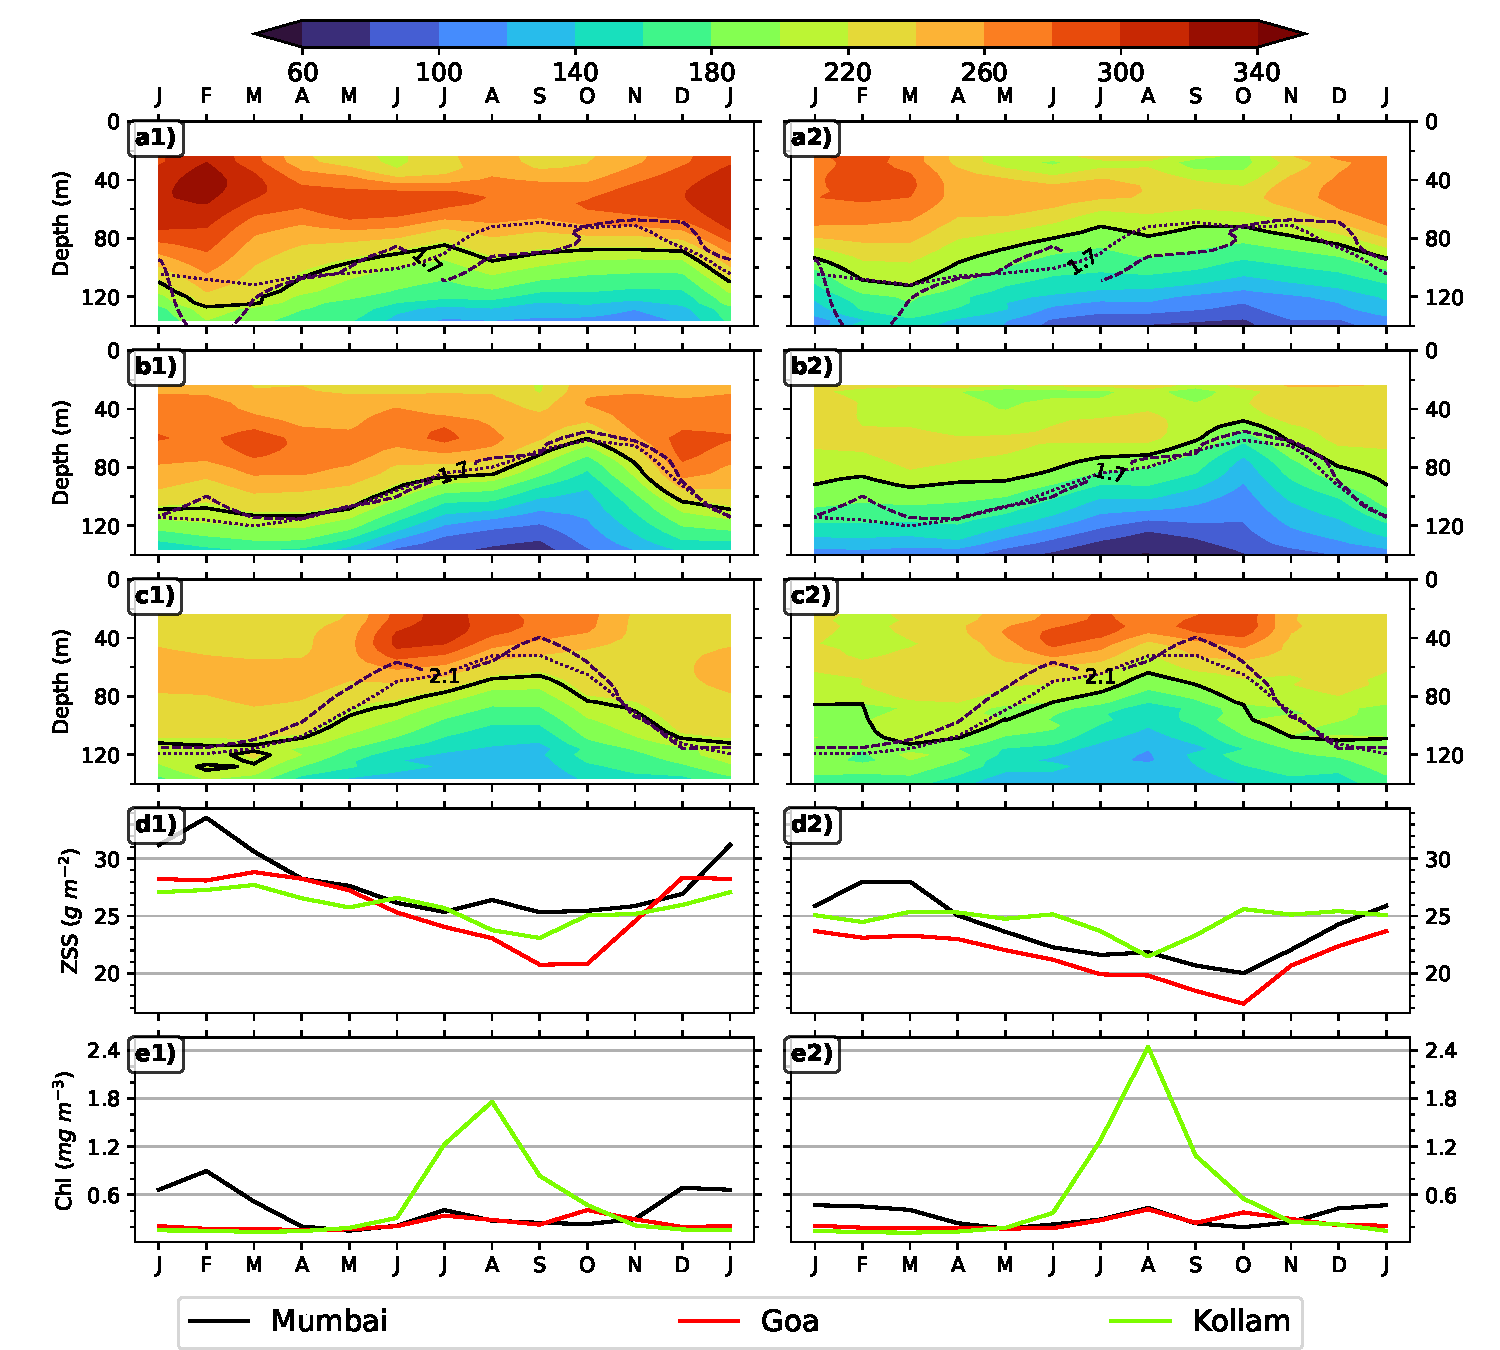
\includegraphics[width=\textwidth]{./fig_s01_climatology_comparison_aparna_ranjan.pdf} 
	\caption{
	Comparison of monthly climatologies from the present dataset (right panel) with those from \citet[A22]{aparna2022seasonal} dataset (left panel). The present dataset spans 2017--2023, while A22's climatology covered 2012--2020. The top panels display the monthly zooplankton biomass climatology for (a1, a2) Mumbai, (b1, b2) Goa, and (c1, c2) Kollam.  The solid black line represents the 215 mg m$^{-3}$ contour (D215), the dotted line indicates the 23$^\circ$C isotherm depth, and dashed lines show oxygen contours.  Panels d1 and d2 illustrate ZSS climatology (integrated over 24--140 m), while e1 and e2 show \chla\ climatology. Note that A22 used SeaWiFS data for \chla, whereas the present study uses L4 \chla\ data from \href{https://doi.org/10.48670/moi-00281}{E.~U.~ Copernicus Marine Service Information}.  Although recent lower biomass off Goa introduces a bias relative to the A22 climatology, the overall climatological patterns remain consistent between the two periods. }
	\label{fig:zsschlclimcomp}
\end{figure}

\begin{figure}[htbp]
	\centering
	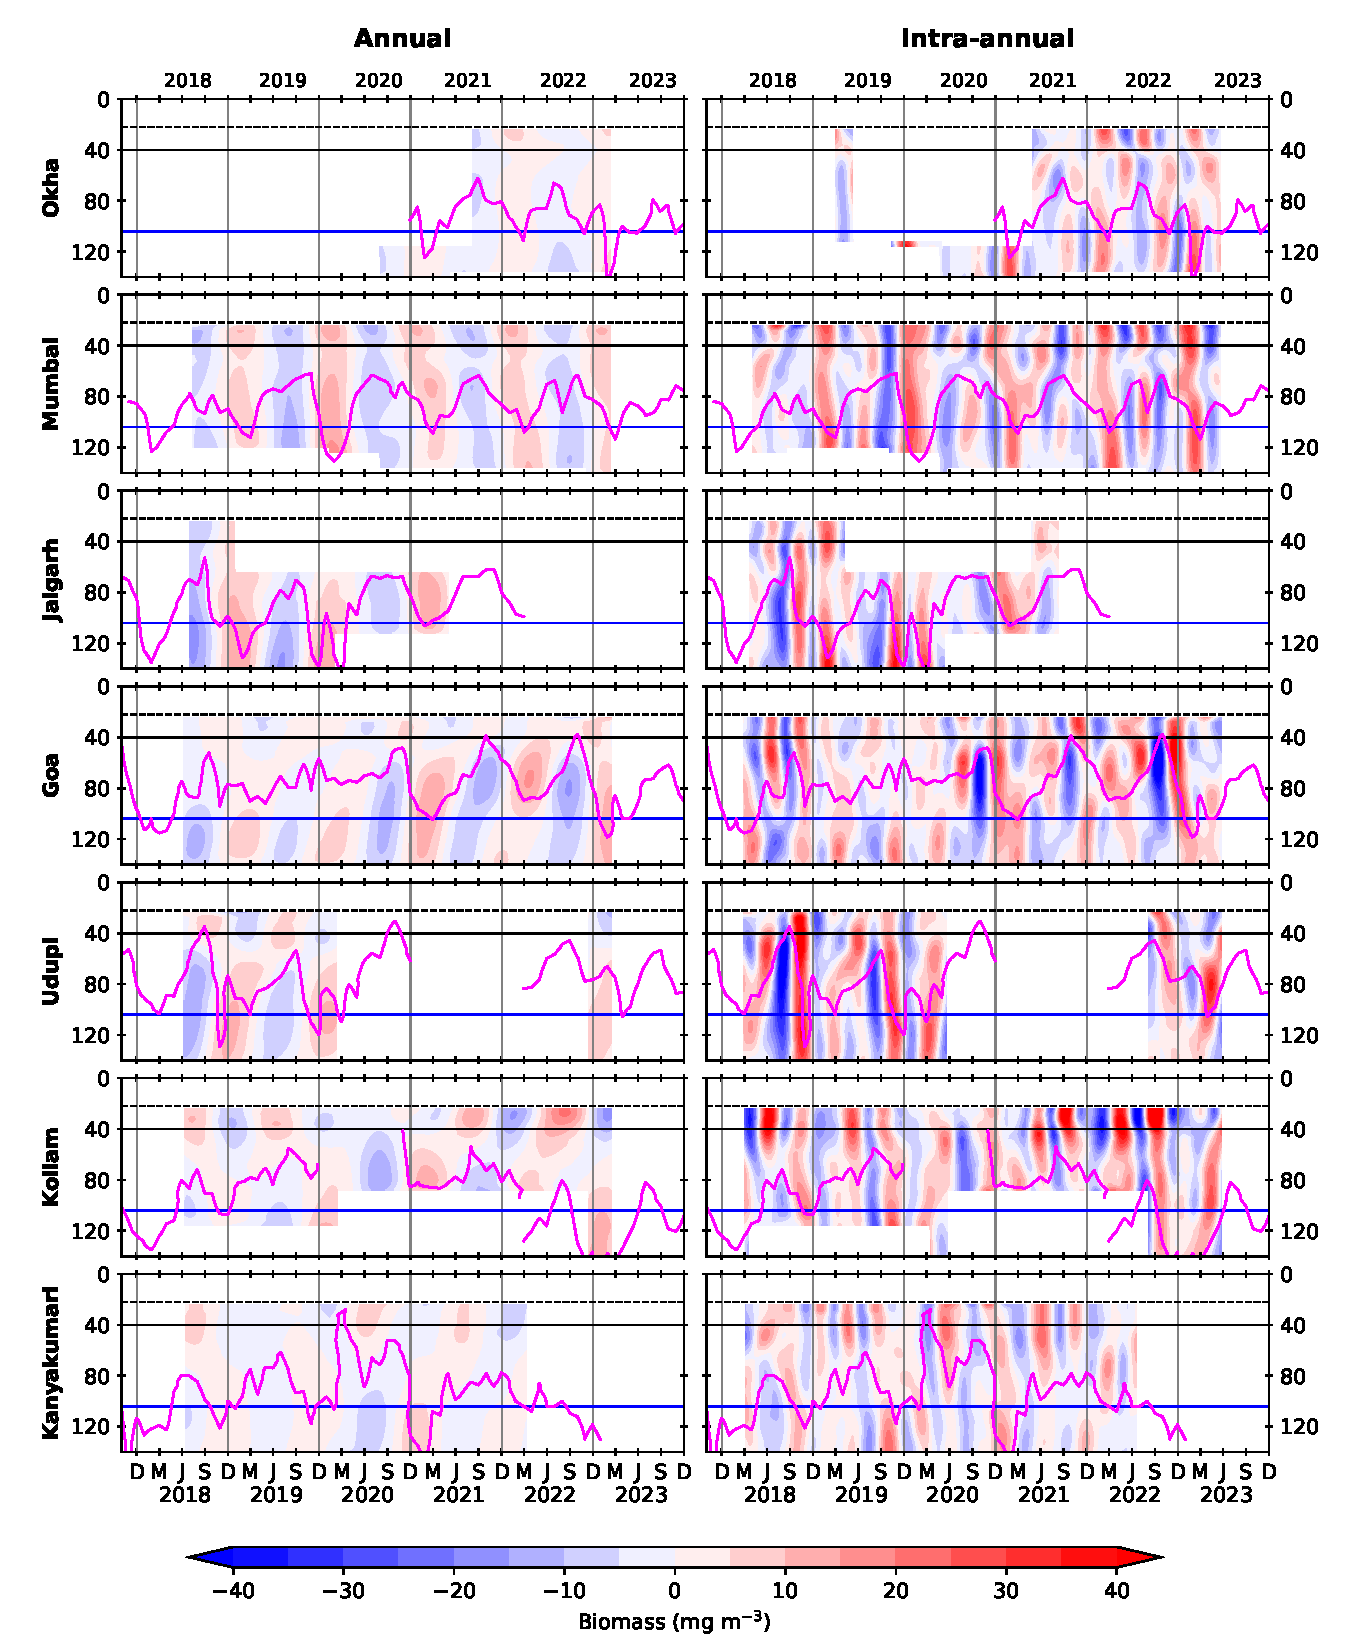
\includegraphics[width=\textwidth]{./fig_s02_filtered_biomass_annual_intraannual.pdf} 
	\caption{Biomass variability (mg m$^{-3}$) extracted using a band-pass filter for all locations.  The left panel depicts the annual cycle (300--400 days) and the right panel shows the intra-annual variability (100--250 days). Horizontal solid black line and solid blue line represent 40~m and 104~m depths, respectively. The vertical black line separate the years. The dashed black line at 22~m marks the upper edge of the first bin (24~m), and the solid magenta curves denote $D215$ (or $D175$ off Okha and Kanyakumari), derived from the monthly biomass time series. The figure demonstrates that the intra-annual variability is stronger than the annual cycle at all locations.}
	\label{fig:intraannual_annual}
\end{figure}

%\begin{figure}[htbp]
%	\centering
%	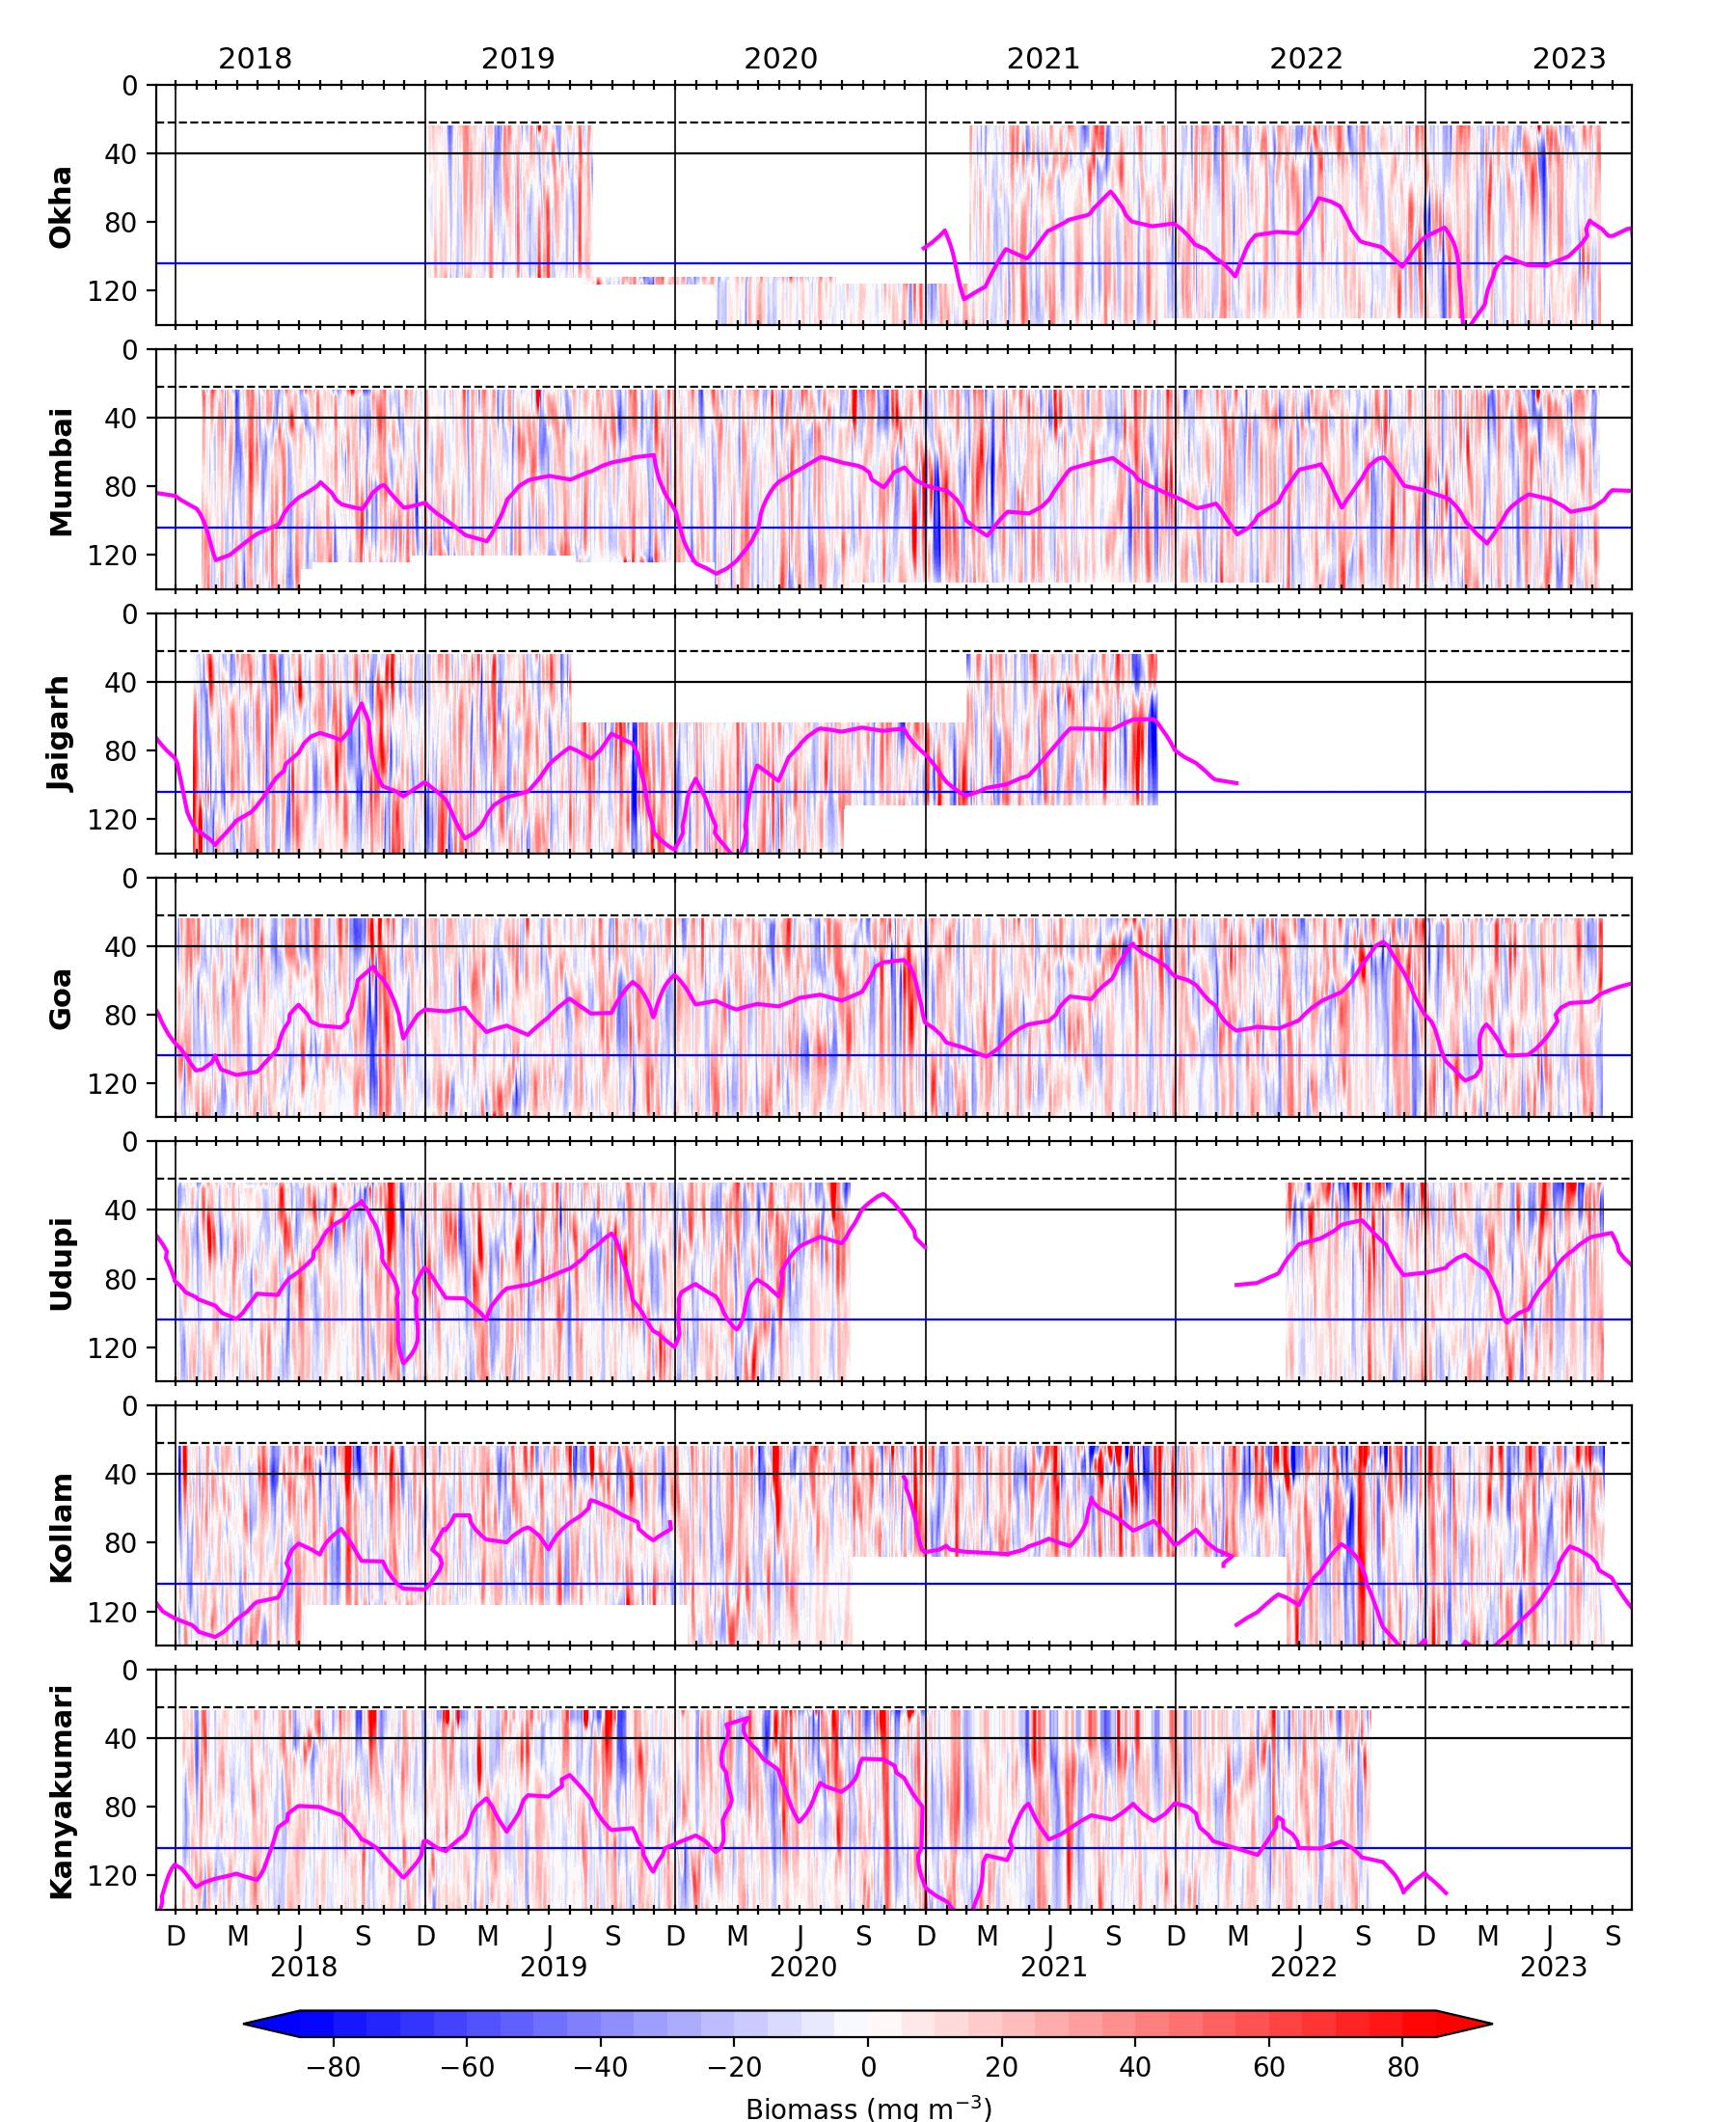
\includegraphics[width=\textwidth]{./filtered_biomass_intraseasonal_5_90days.pdf} 
%	\caption{Biomass variation in intraseasonal band i.e., 5 to 90 days period is obtained using a lanczos band pass filter, It includes both the high- and low-frequency components. The horizontal black and blue lines is for 40 and 104 m, vertical black lines separate the years and solid magenta curves denote $D215$ ($$D175$$ off Okha and Kanyakumari) fetched from monthly biomass. The dashed line at 22 m marks the top-depth of first bin i.e, 24 m. Intraseasonal variability is seen throughout the record, and it is coherent along the slope, e.~g, during October--December 2018.}
%	\label{fig:filtered_biomass_intraseasonal_5_90days_2019}
%\end{figure}

\begin{figure}[htbp]
	\centering
	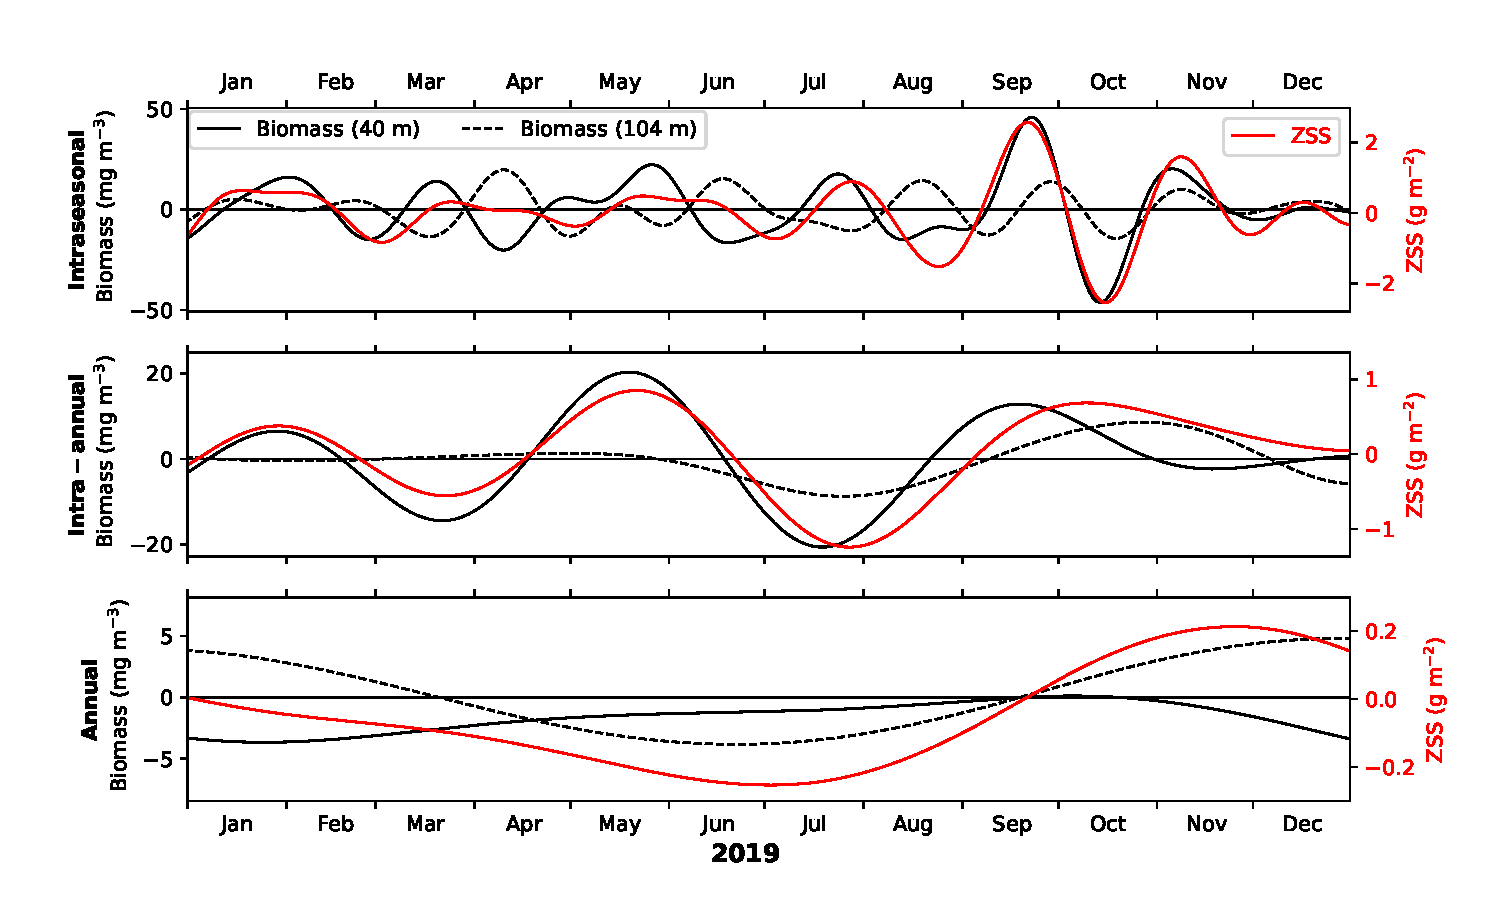
\includegraphics[width=\textwidth]{./fig_s03_ss_biomass_comparison_intraseasonal_band.pdf} 
	\caption{The figure compares band-passed filtered biomass (mg m$^{-3}$) at 40~m  and 104~m with ZSS (g m$^{-2}$), integrated over 24--120 m, from Kanyakumari during 2019. Biomass at 40 m is shown as a black solid line, at 104 m as a black dashed line, while ZSS is a red solid line. The top panel illustrates intraseasonal biomass (30–90 days), the middle panel shows intra-annual biomass (100–250 days), and the bottom panel displays the annual biomass cycle (300–400 days).  The comparison shows that the biomass at 104~m is frequently out of phase with upper-ocean biomass at 40~m across all three time scales. This phase difference between surface and subsurface biomass can either enhance or reduce the overall ZSS.}
	\label{fig:40_104_biomass_zss}
\end{figure}

\begin{figure}[htbp]
		\centering
		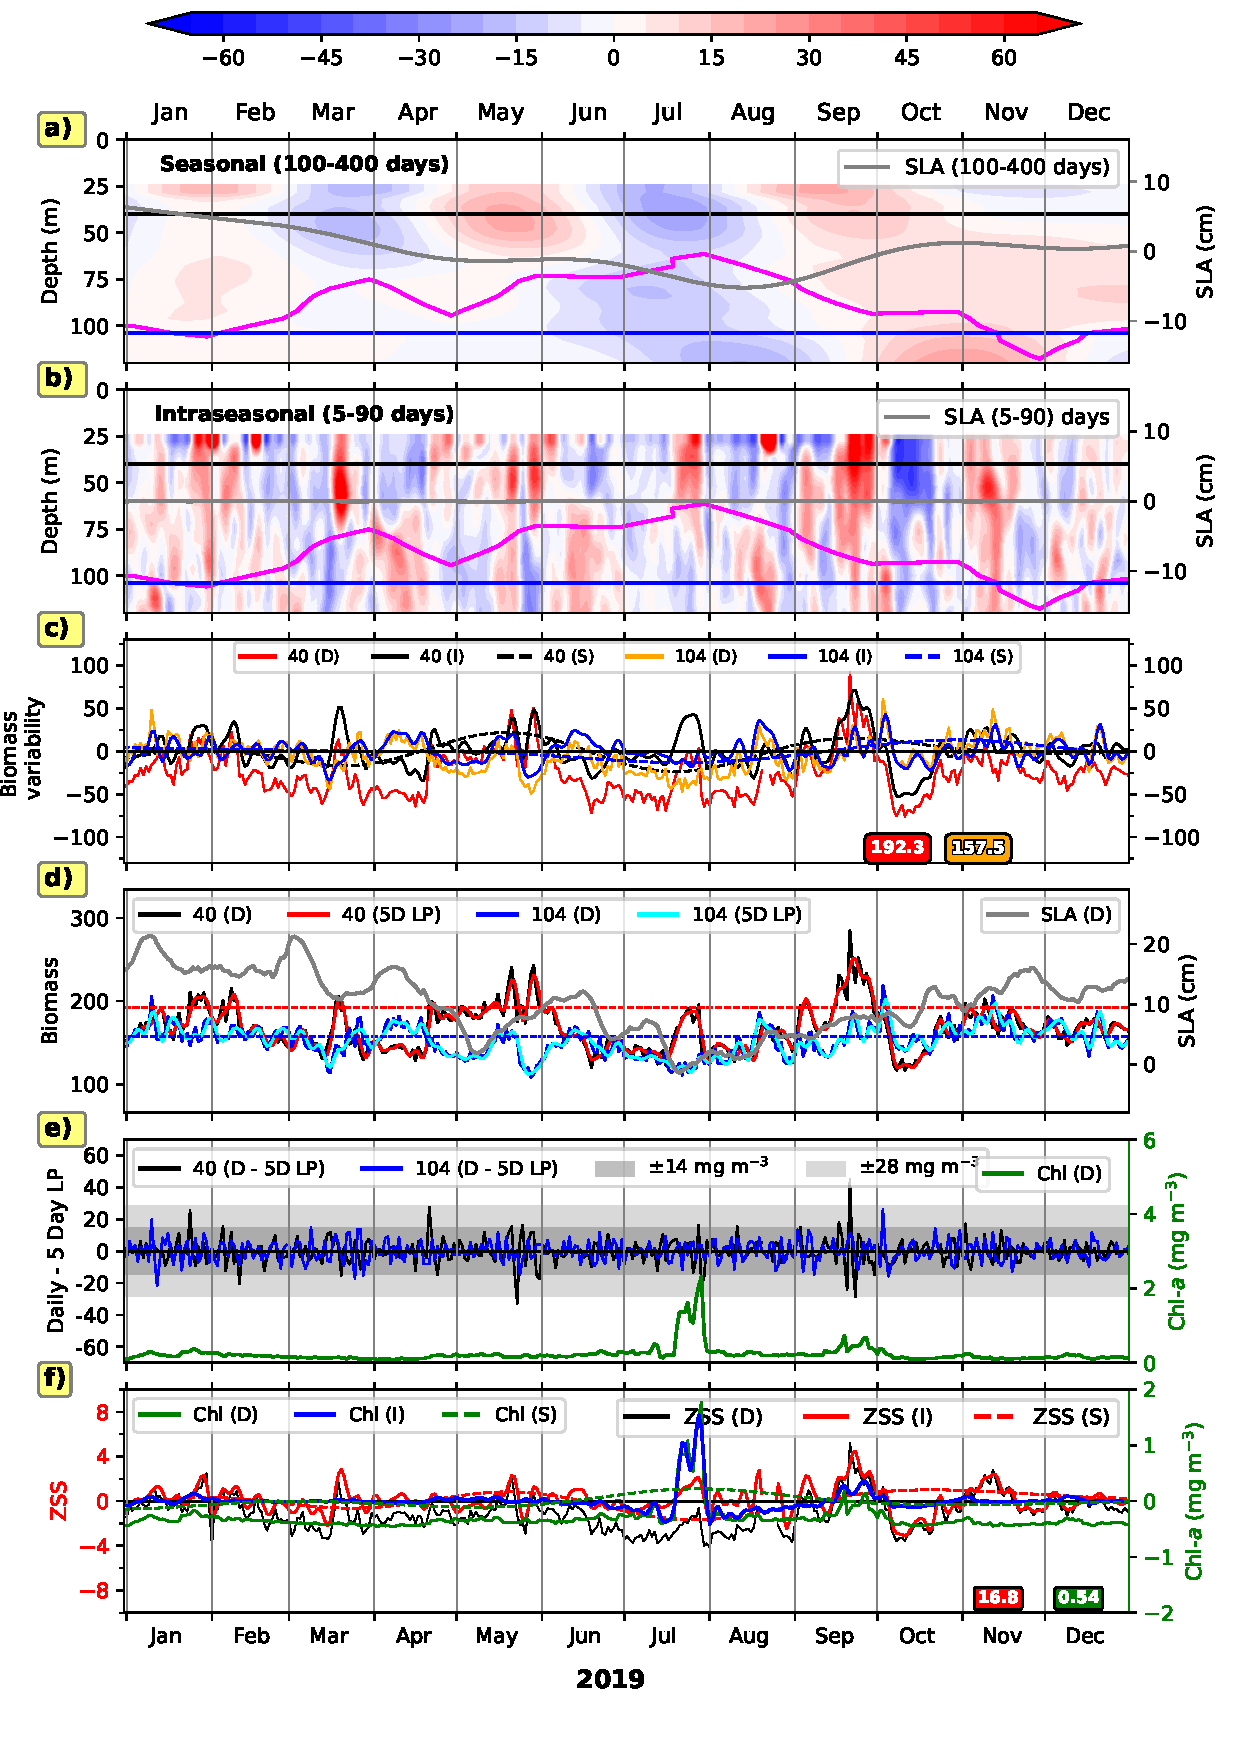
\includegraphics[width=0.78\textwidth]{./fig_s04_biomass_intra_2019_kanyakumari.pdf}
		\caption{The figure shows a comparison of biomass variability (mg m$^{-3}$) in the seasonal (100–400 days) and intraseasonal (5–90 days) bands off Kanyakumari for the year 2019. For all panels, vertical grey lines separate the months. Panels (a) and (b) present time-depth plots of seasonal and intraseasonal biomass, respectively. Overlaid grey contours represent the corresponding sea level anomaly (SLA). Biomass at 40 m and 104 m depths is marked by black and blue horizontal lines. The magenta curves denote D175. Panel (c) shows the daily, intraseasonal, and seasonal biomass at 40 m and 104 m. The mean of the daily biomass time series for 40 m (red) and 104 m (orange) is indicated in the bottom right corner of this panel. Panel (d) compares daily SLA (grey) with daily and 5-day low-pass filtered biomass at 40 m and 104 m. Panel (e) illustrates the difference between daily and 5-day low-pass filtered biomass at both depths. Grey and light grey shaded regions denote the $\pm 1$ SD and $\pm 2$ SD bounds, respectively, derived from the backscatter-biomass relationship. Daily \chla\ (green) is overlaid onto this panel. The bottom panel (f) shows daily satellite \chla\ and ZSS, and their variability in the intraseasonal and seasonal bands.}
		\label{fig:biomass_intra_2019_kanyakumari}

\end{figure}

\begin{figure}[htbp]
	\centering
	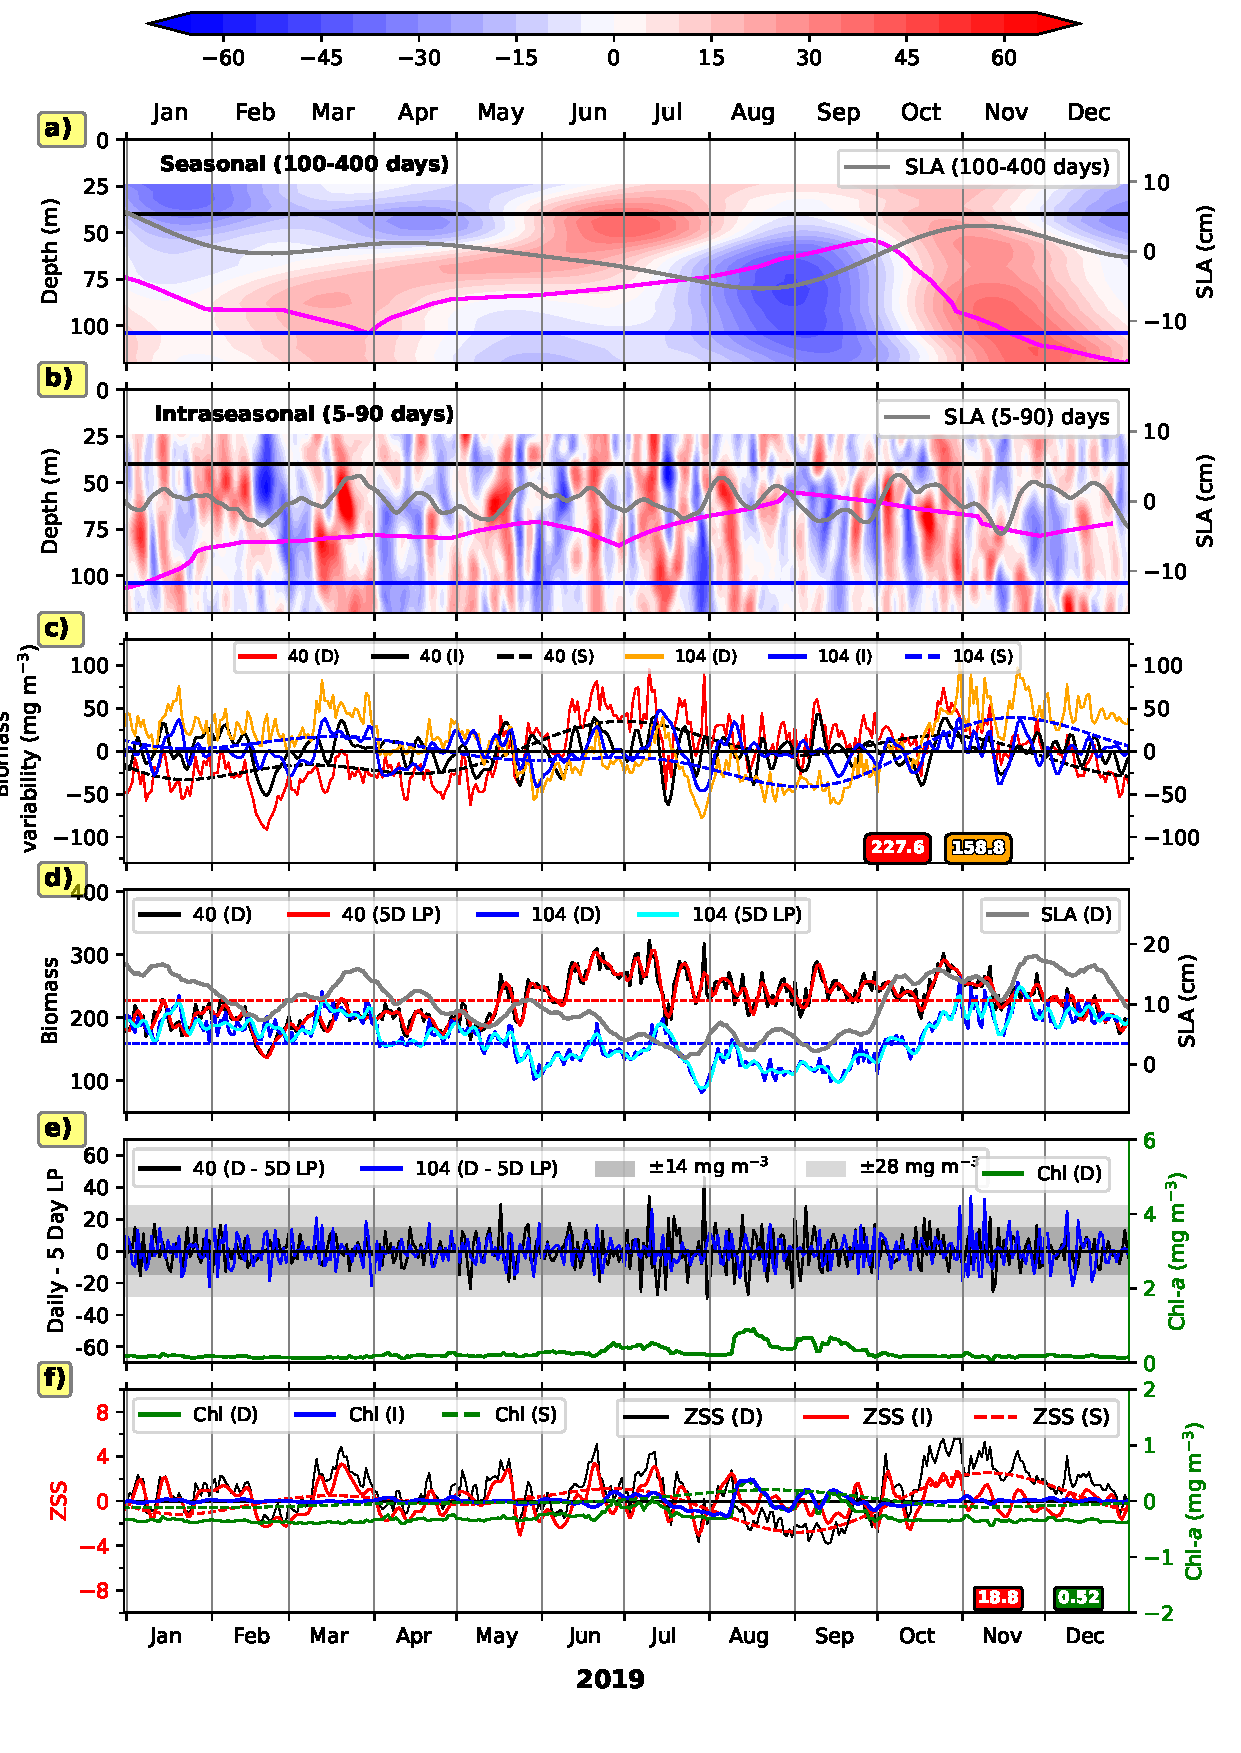
\includegraphics[width=0.8\textwidth]{./fig_s05_biomass_intra_2019_udupi.pdf} 
	\caption{Same as in Fig.~\ref{fig:biomass_intra_2019_kanyakumari} but for Udupi with $D215$ curve in top two panels.}		
	\label{fig:biomass_intra_2019_udupi}
\end{figure}

\begin{figure}[htbp]
	\centering
	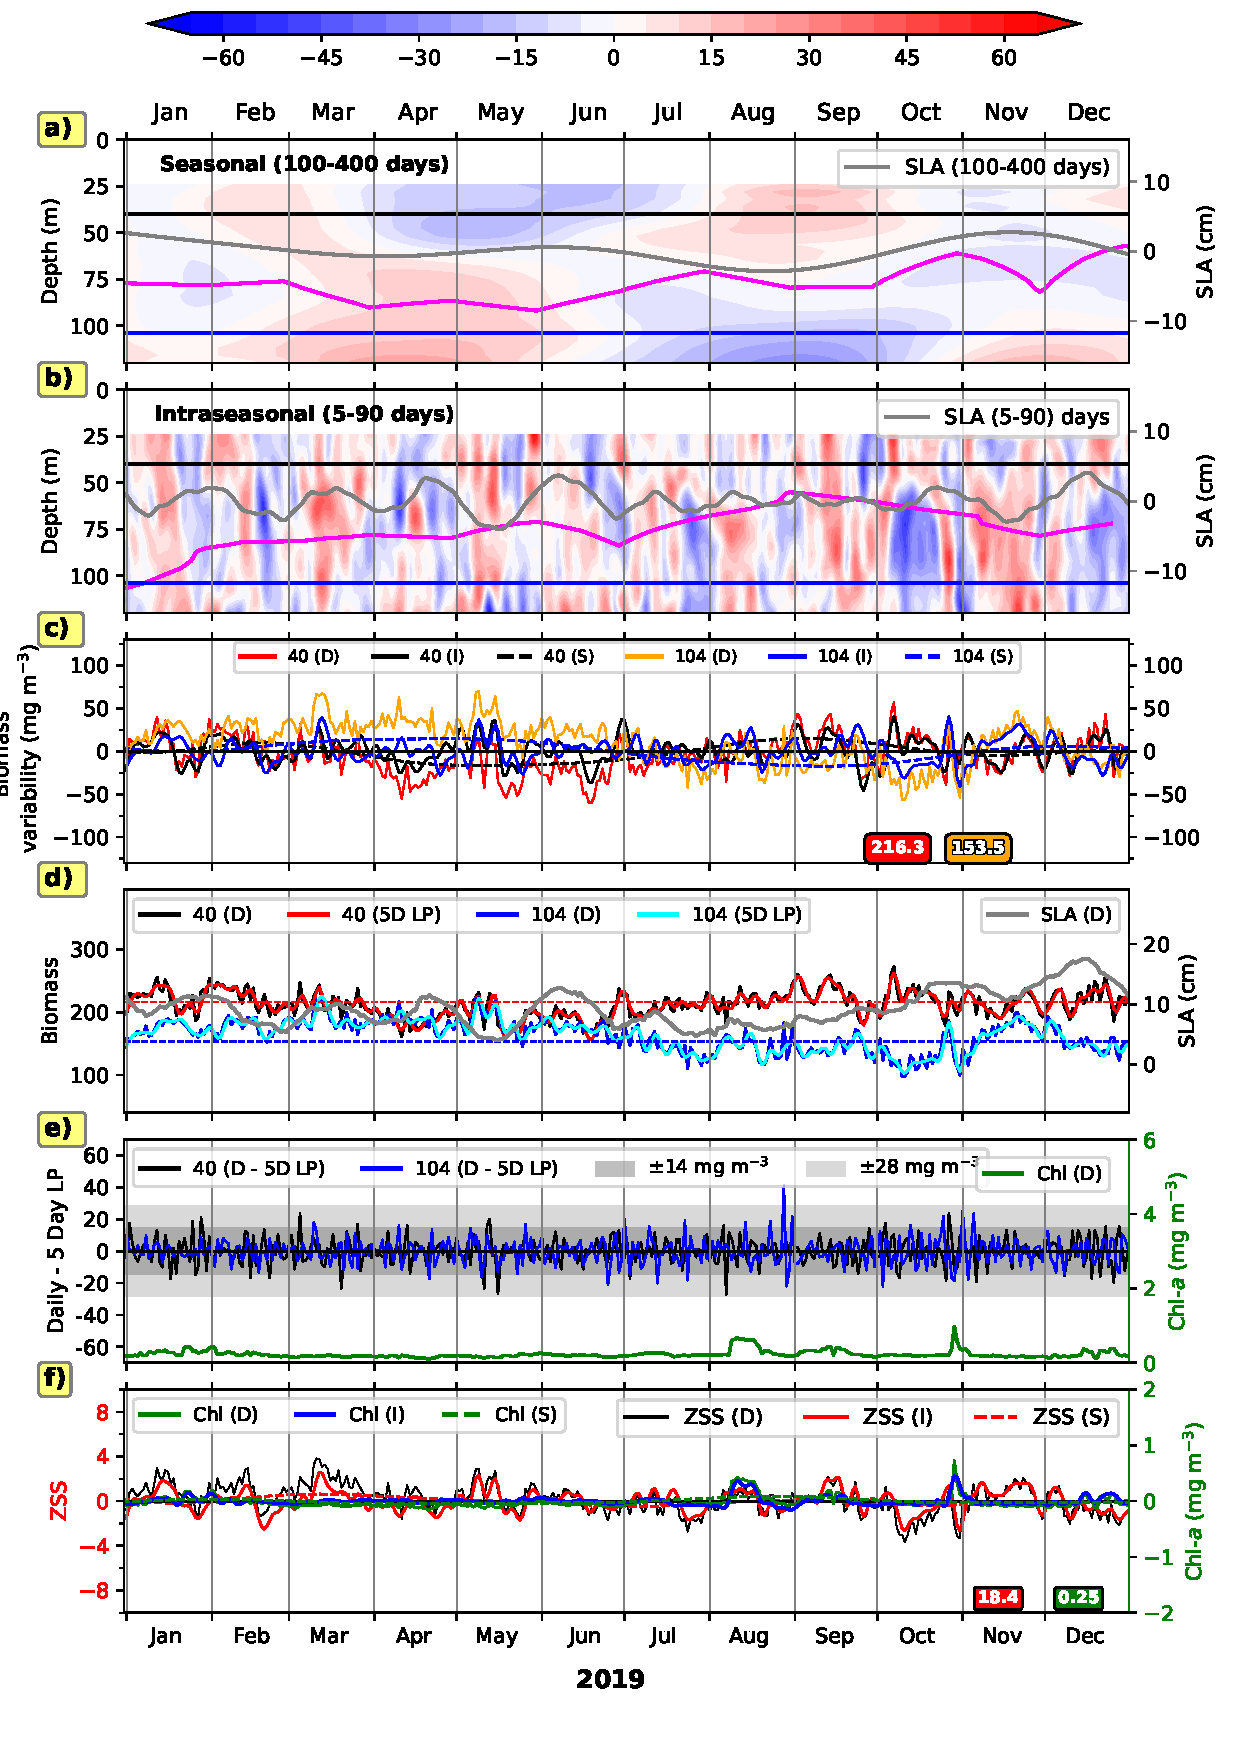
\includegraphics[width=0.8\textwidth]{./fig_s06_biomass_intra_2019_goa.pdf} 
	\caption{Same as in Fig.~\ref{fig:biomass_intra_2019_kanyakumari} but for Goa with $D215$ curve in top two panels.}		
	\label{fig:biomass_intra_2019_goa}
\end{figure}


\begin{figure}[htbp]
	\centering
	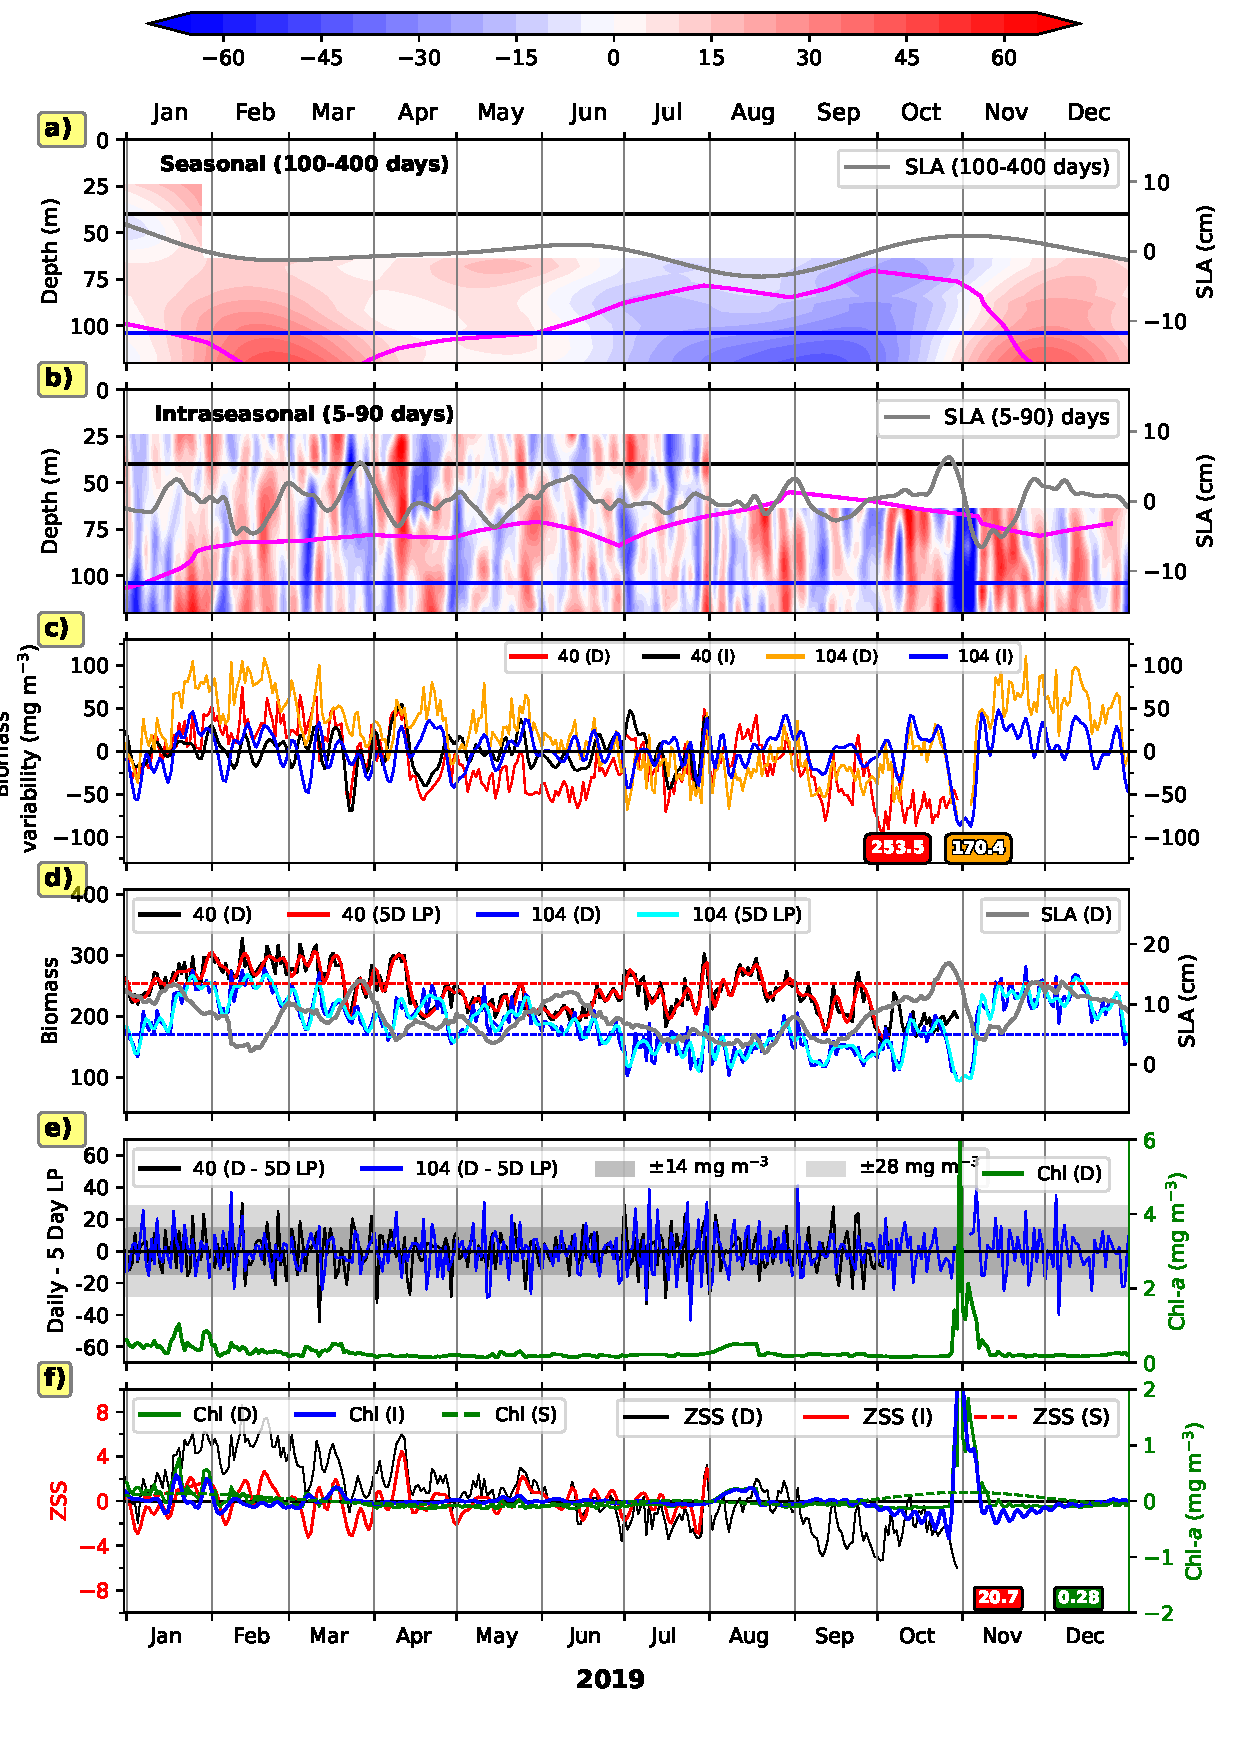
\includegraphics[width=0.8\textwidth]{./fig_s07_biomass_intra_2019_jaigarh.pdf} 
	\caption{Same as in Fig.~\ref{fig:biomass_intra_2019_kanyakumari} but for Jaigarh with $D215$ curve in top two panels.}		
	\label{fig:biomass_intra_2019_jaigarh}
\end{figure}

\begin{figure}[htbp]
	\centering
	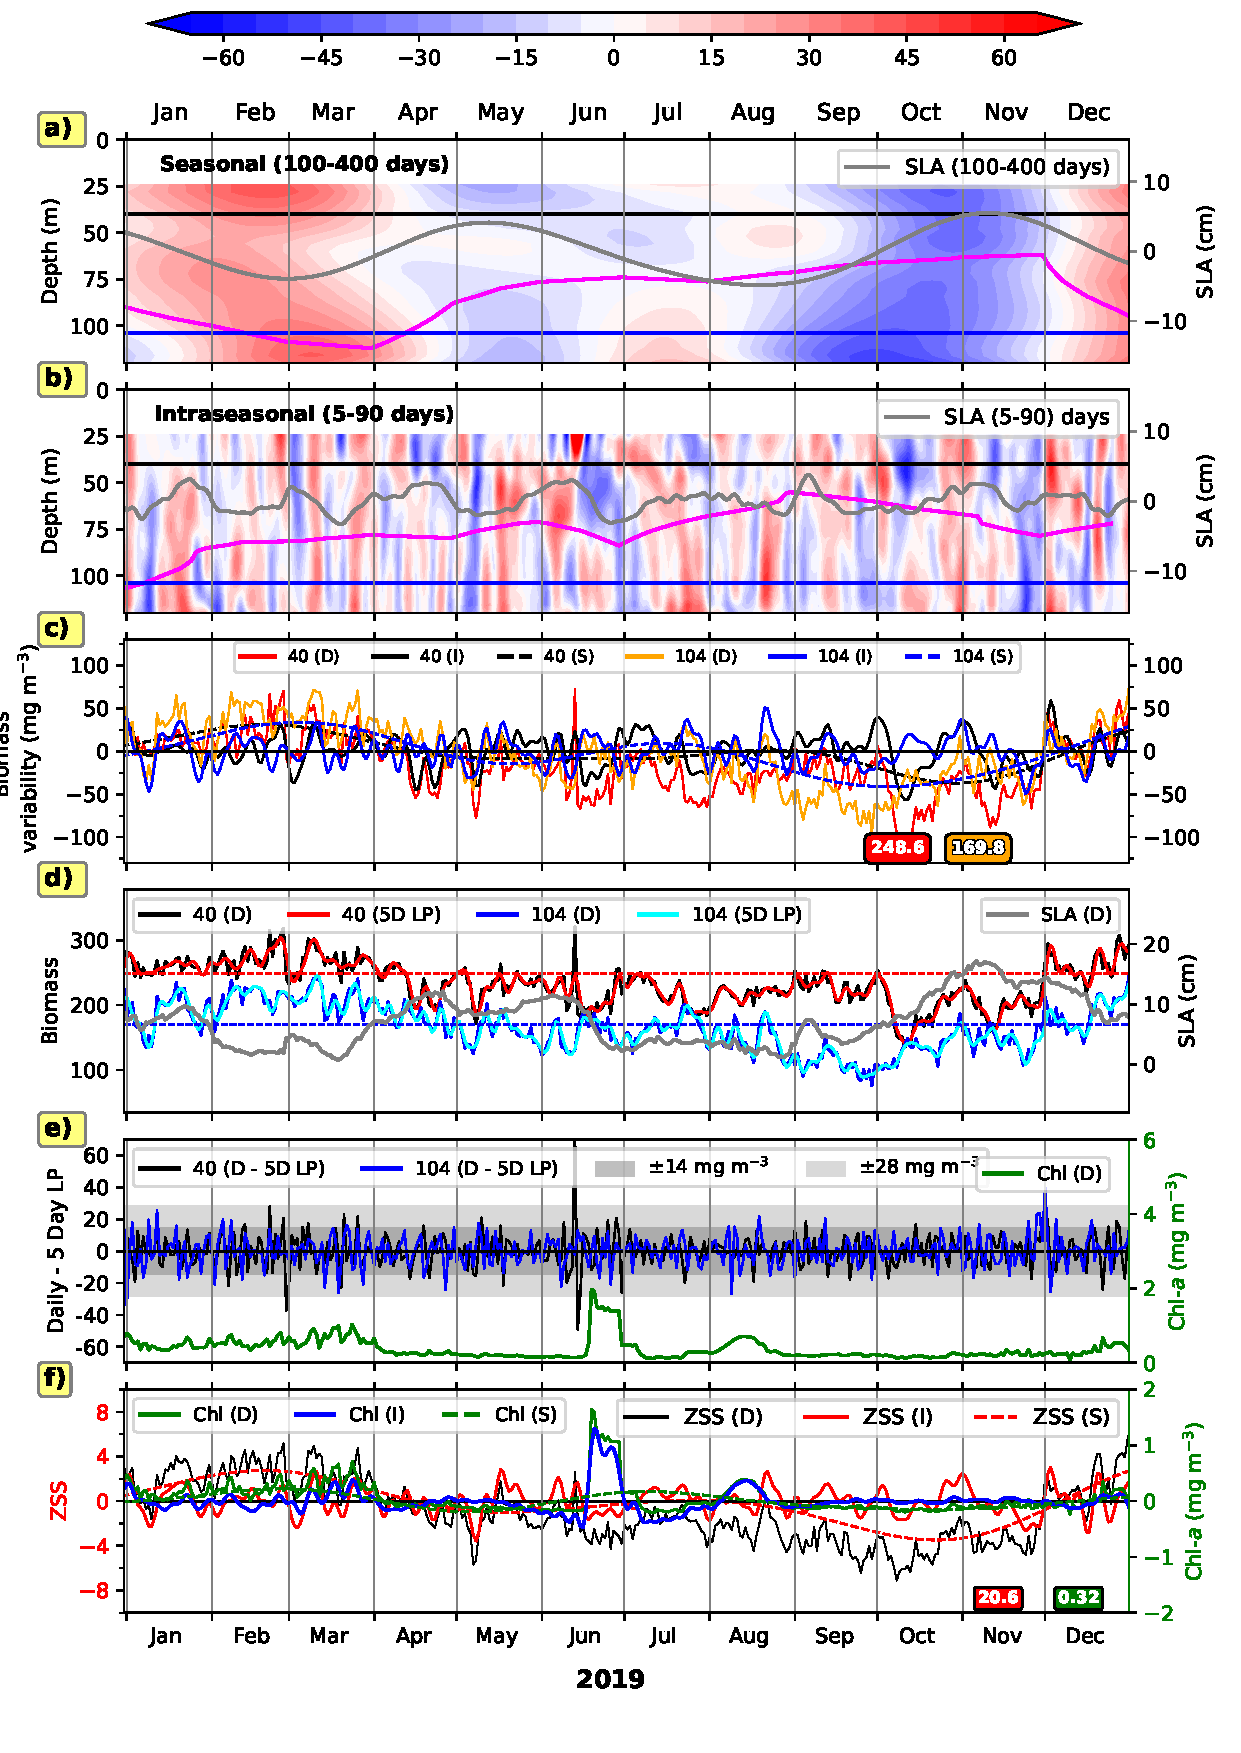
\includegraphics[width=0.8\textwidth]{./fig_s08_biomass_intra_2019_mumbai.pdf} 
	\caption{Same as in Fig.~\ref{fig:biomass_intra_2019_kanyakumari} but for Mumbai with $D215$ curve in top two panels.}		
	\label{fig:biomass_intra_2019_mumbai}
\end{figure}

\begin{figure}[htbp]
	\centering
	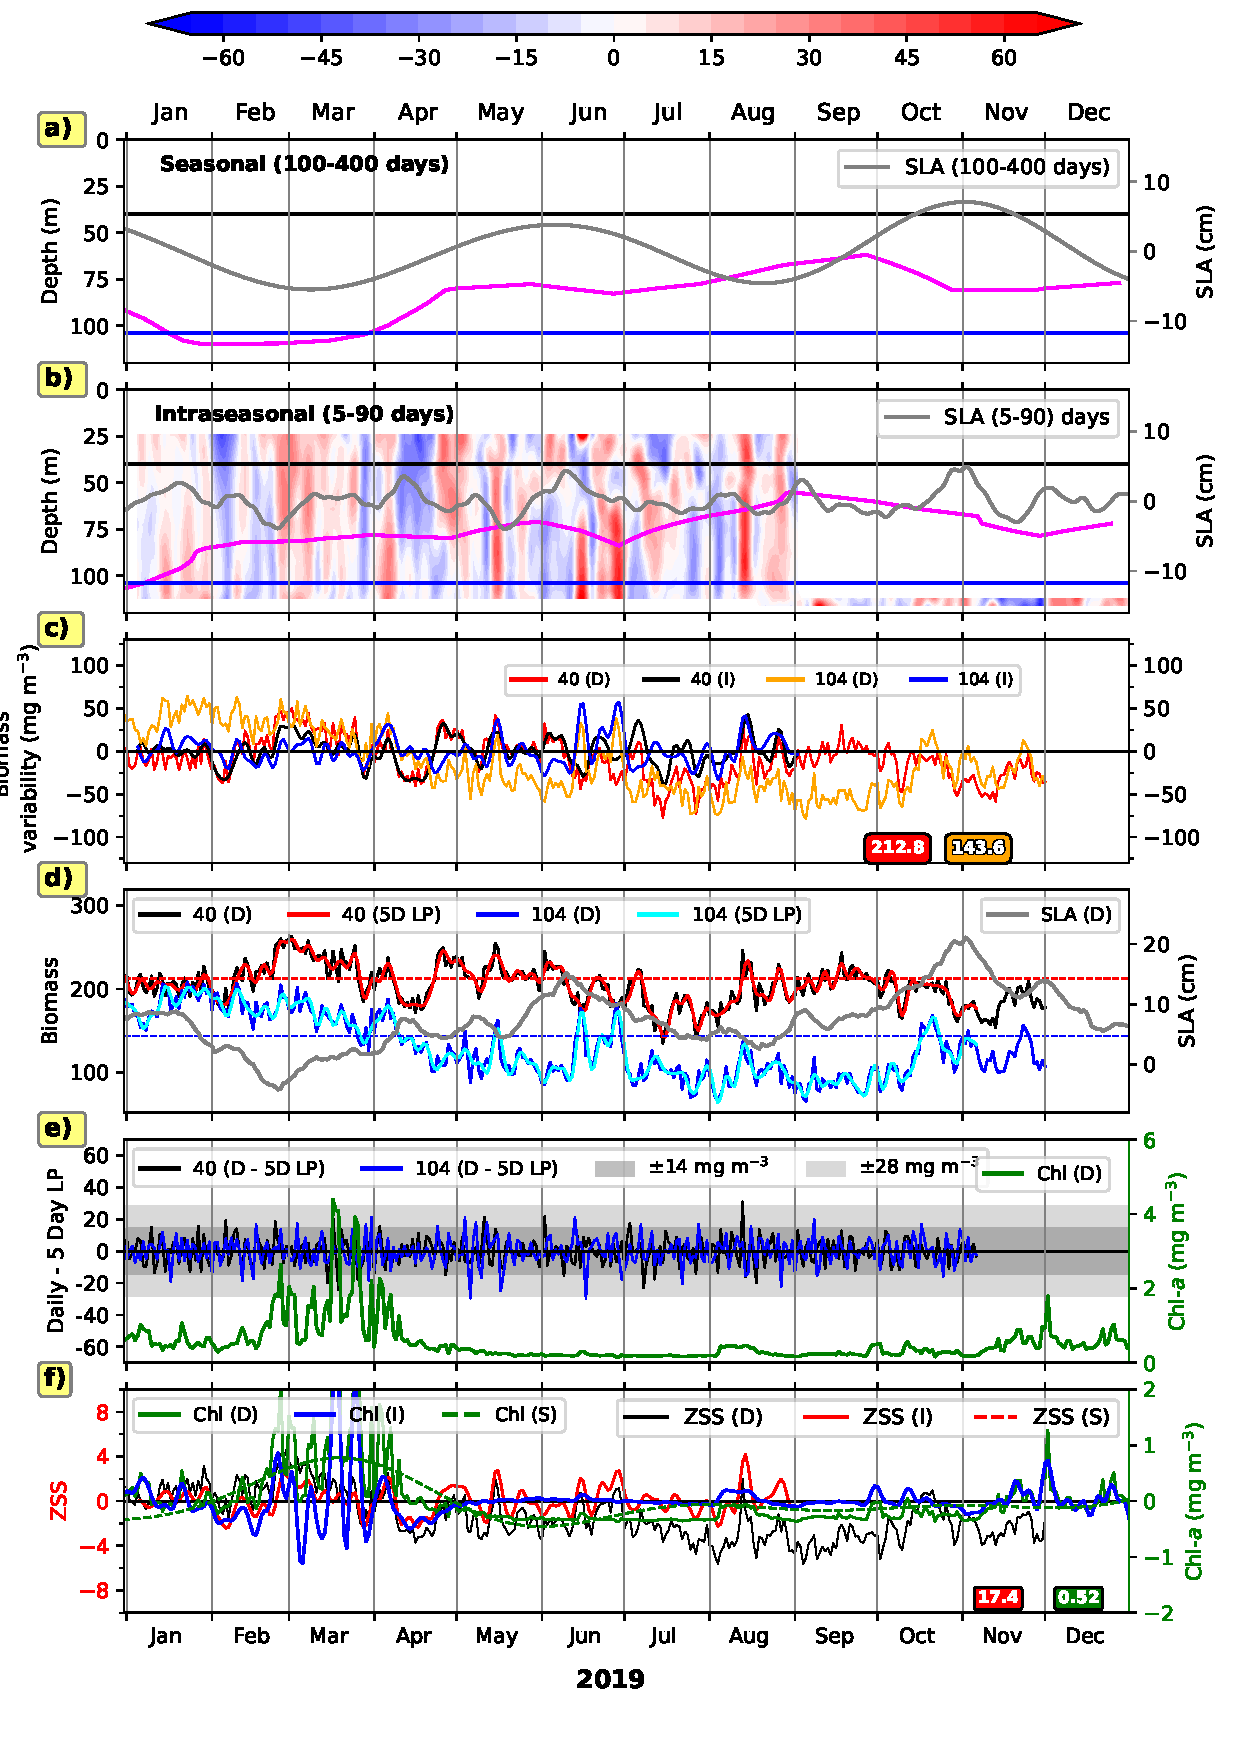
\includegraphics[width=0.8\textwidth]{./fig_s09_biomass_intra_2019_okha.pdf} 
	\caption{Same as in Fig.~\ref{fig:biomass_intra_2019_kanyakumari} but for Okha with $D175$ curve in top two panels.}		
	\label{fig:biomass_intra_2019_okha}
\end{figure}


\begin{figure}[htbp]
	\centering
	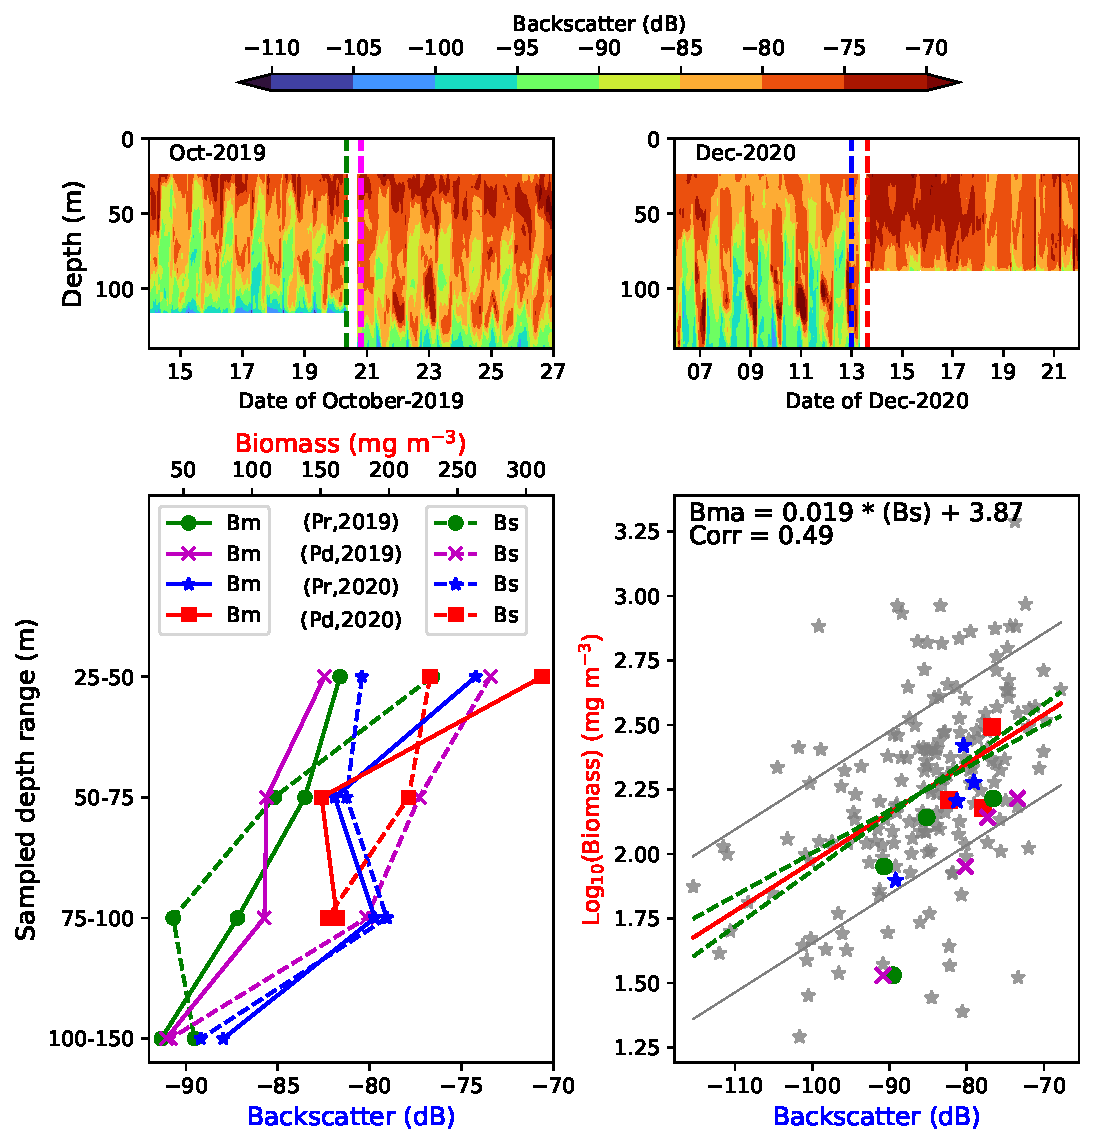
\includegraphics[width=\textwidth]{./fig_s10_Kollam_2020_verification.pdf} 
	\caption{The figure presents Kollam ADCP backscatter (Bs) and its relationship with biomass data (mg m$^{-3}$) obtained from volumetric zooplankton samples collected during during 2019 and 2020. The top panels display ADCP backscatter data before retrieval and after deployment. Specifically, the top-left (top-right) panel shows biomass data for October 2019 (December 2020), with retrieval and redeployment times marked by dashed green (blue) and dashed purple (red) vertical lines, respectively. The bottom-left panel shows biomass profiles (Bm) from zooplankton samples (solid lines), collected over selected sampling depth ranges, and corresponding ADCP backscatter profiles, integrated over the same depth ranges (dashed lines). These profiles are shown for the pre-retrieval (Pr) and post-deployment (Pd) phases of both 2019 and 2020. The bottom-right panel displays biomass (log$_{10}$ scale) plotted against backscatter from 2017 to 2023 for data from all seven stations. The ADCP backscatter derived biomass (Bma) is obtained using a linear regression line fitted between zooplankton biomass and ADCP backscatter. Data for Kollam in 2019 and 2020 are highlighted, with symbols and colors in this panel corresponding to those in the bottom-left panel.}
	\label{fig:kollam_verification_2020}
\end{figure}

\begin{figure}[htbp]
	\centering
	\includegraphics[width=\textwidth]{./fig_s11_biomass_spikes_40m.pdf} 
	\caption{The figure illustrates biomass spikes and associated variability using daily time series and filtered data. Panels (a) and (b) show spikes as the difference between the mean-removed daily biomass time series (red) and the 5-day low-pass filtered biomass (black) at 40 m depth, off Jaigarh. Satellite \chla\ is overlaid for the same duration. Note that the ordinates are different for each time series. Shaded regions represent $\pm 1$ SD ($\pm 14$ mg m$^{-3}$, red) and $\pm 2$ SD ($\pm 28$ mg m$^{-3}$, light red) from the mean-removed daily time series. The date of each spike event is noted in the top-right corner of each panel, with red and blue text indicating positive and negative spikes, respectively. The panels in the second row show depth-time plots for hourly biomass data; the black horizontal line marks the depth from which the time series for the top panels are extracted. Similarly, panels (c) and (d) show a positive and a negative spike event off Kollam. The bottom panels show the corresponding depth-time plots for biomass data.}
	\label{fig:biomass_spike_40m}
\end{figure}

\begin{figure}[htbp]
	\centering
	\includegraphics[width=\textwidth]{./fig_s12_biomass_spikes_104m.pdf} 
	\caption{Same as Fig.~\ref{fig:biomass_spike_40m} but for biomass at 104~m depth.}
	\label{fig:biomass_spike_104m}
\end{figure}


\end{document}
